\chapter{Virittävät puut}

\section{Union-find-rakenne}

Union-find-rakenne pitää yllä alkioiden joukkoja ja tarjoaa
seuraavat tehokkaat operaatiot:

\begin{itemize}
\item yhdistä kaksi joukkoa samaksi joukoksi
\item tarkista, ovatko kaksi alkiota samassa joukossa
\end{itemize}

Tarkastellaan esimerkkinä tilannetta, jossa joukot ovat
$A=\{1,4\}$, $B=\{2,5,6\}$ ja $C=\{3,7,8\}$.
Tällä hetkellä alkiot $1$ ja $2$ ovat eri joukoissa.
Yhdistämme sitten joukot $A$ ja $B$,
jolloin niistä syntyy joukko $\{1,2,4,5,6\}$.
Tämän jälkeen alkiot $1$ ja $2$ ovat samassa joukossa.

Verkkojen tapauksessa voimme tulkita operaatiot näin:

\begin{itemize}
\item lisää kaari kahden erillisen komponentin välille
\item tarkista, ovatko kaksi solmua samassa komponentissa
\end{itemize}

\begin{figure}
\center
\begin{center}
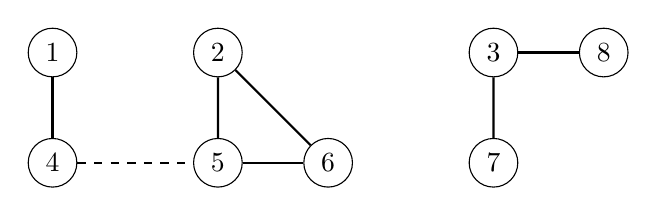
\begin{tikzpicture}[scale=0.7]
\node[draw, circle] (1) at (0,0) {$1$};
\node[draw, circle] (4) at (0,-2) {$4$};

\node[draw, circle] (2) at (3,0) {$2$};
\node[draw, circle] (5) at (3,-2) {$5$};
\node[draw, circle] (6) at (5,-2) {$6$};

\node[draw, circle] (3) at (8,0) {$3$};
\node[draw, circle] (7) at (8,-2) {$7$};
\node[draw, circle] (8) at (10,0) {$8$};

\path[draw,thick,-] (1) -- (4);
\path[draw,thick,-] (2) -- (5);
\path[draw,thick,-] (2) -- (6);
\path[draw,thick,-] (5) -- (6);
\path[draw,thick,-] (3) -- (7);
\path[draw,thick,-] (3) -- (8);

\path[draw,thick,-,dashed] (4) -- (5);
\end{tikzpicture}
\end{center}
\caption{Verkon komponentit ovat $\{1,4\}$, $\{2,5,6\}$ ja $\{3,7,8\}$.
Kun lisäämme kaaren $4-5$, kaksi komponenttia yhdistyy.}
\label{fig:veryhd}
\end{figure}

Kuvassa \ref{fig:veryhd} on äskeistä esimerkkiä vastaava tilanne verkkona.
Kun li\-säämme kaaren solmujen $4$ ja $5$ välille,
kaksi komponenttia yhdistyy ja solmut $1$ ja $2$
ovat samassa komponentissa.

\subsection{Rakenteen toteutus}

Toteutamme union-find-rakenteen niin, että jokaisessa joukossa
yksi alkioista on joukon \emph{edustaja} ja muut alkiot viittaavat
edustajaan suoraan tai muiden alkioiden kautta.
Kun haluamme tarkastaa, ovatko kaksi alkiota samassa joukossa,
selvitämme niiden edustajat ja vertaamme niitä toisiinsa.

Jokaisella joukon alkiolla $x$ on arvo $\texttt{next}[x]$,
joka kertoo seuraavan alkion viittauksien ketjussa.
Jos $\texttt{next}[x]=x$, alkio on joukon edustaja.
Tämän ansiosta saamme selville mille tahansa alkiolle $x$,
mikä on vastaavan joukon edustaja, kulkemalla läpi viittausten ketjun.

\begin{figure}
\center
\begin{center}
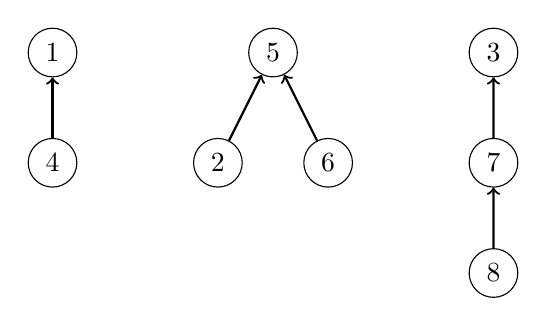
\begin{tikzpicture}[scale=0.7]
\node[draw, circle] (1) at (0,0) {$1$};
\node[draw, circle] (4) at (0,-2) {$4$};

\node[draw, circle] (2) at (3,-2) {$2$};
\node[draw, circle] (5) at (4,0) {$5$};
\node[draw, circle] (6) at (5,-2) {$6$};

\node[draw, circle] (3) at (8,0) {$3$};
\node[draw, circle] (7) at (8,-2) {$7$};
\node[draw, circle] (8) at (8,-4) {$8$};

\path[draw,thick,->] (4) -- (1);
\path[draw,thick,->] (2) -- (5);
\path[draw,thick,->] (6) -- (5);
\path[draw,thick,->] (7) -- (3);
\path[draw,thick,->] (8) -- (7);
\end{tikzpicture}
\end{center}
\caption{Union-find-rakenne, joka vastaa joukkoja $\{1,4\}$, $\{2,5,6\}$ ja $\{3,7,8\}$.}
\label{fig:unifin}
\end{figure}

Kuvassa \ref{fig:unifin} on esimerkki union-find-rakenteesta, kun joukot ovat
$A=\{1,4\}$, $B=\{2,5,6\}$ ja $C=\{3,7,8\}$.
Joukkojen edustajat ovat 1, 5 ja 3.
Esimerkiksi $\texttt{next}[1]=1$ ja $\texttt{next}[2]=5$.
Saamme selville alkion 8 joukon edustajan kulkemalla ketjua
$8 \rightarrow 7 \rightarrow 3$.

Seuraava operaatio \texttt{find} selvittää alkion $x$ joukon edustajan:

\begin{code}
int find(int x) {
    while (x != next[x]) {
        x = next[x];
    }
    return x;
}
\end{code}

Tämän avulla voimme luoda operaation \texttt{same}, joka tarkastaa,
ovatko alkiot $a$ ja $b$ samassa joukossa.
Alkiot ovat samassa joukossa täsmälleen silloin, kun niillä
on sama edustaja:

\begin{code}
boolean same(int a, int b) {
    return find(a) == find(b);
}
\end{code}

Viimeinen tarvittava operaatio on \texttt{union}, joka yhdistää alkioita
$a$ ja $b$ vastaavat joukot.
Yksinkertainen tapa toteuttaa operaatio on seuraava:

\begin{code}
void union(int a, int b) {
    a = find(a);
    b = find(b);
    next[a] = b;
}
\end{code}

Tässä toteutuksessa selvitämme ensin kummankin joukon edustajat,
ja sitten asetamme ensimmäisen edustajan viittaamaan toiseen.

Tässä kuvattu tapa toteuttaa union-find-rakenne on toimiva,
mutta se \emph{ei} ole tehokas.
Ongelmana on, että \texttt{union}-operaatiot saattavat tuottaa
pitkän viittausten ketjun, jolloin \texttt{find}- ja
\texttt{same}-operaatiot toimivat hitaasti.
Pahimmassa tapauksessa kaikki $n$ alkiota voivat olla
samassa ketjussa, jolloin operaatiot vievät aikaa $O(n)$.
Seuraavaksi toteutammekin rakenteen paremmin niin,
että pitkiä ketjuja ei pääse syntymään.

\subsection{Tehokas yhdistäminen}

Osoittautuu, että saamme aikaan tehokkaan union-find-rakenteen,
kunhan toteutamme kahden joukon yhdistämisen niin,
että asetamme \emph{pienemmän} joukon edustajan viittaamaan
\emph{suuremman} joukon edustajaan. Jos joukot ovat yhtä suuria,
voimme valita kummin vain.

Tätä varten pidämme jokaiselle alkiolle $x$ yllä tietoa
$\texttt{size}[x]$: jos alkio $x$ on joukon edustaja,
kuinka monta alkiota joukossa on.
Kuvassa \ref{fig:unifin} esimerkiksi $\texttt{size}[1]=2$
ja $\texttt{size}[5]=3$.
Huomaa, että jos solmu $x$ ei ole joukon edustaja,
arvo $\texttt{size}[x]$ ei sisällä oikeaa tietoa.

Nyt voimme toteuttaa joukkojen yhdistämisen näin:

\begin{code}
void union(int a, int b) {
    a = find(a);
    b = find(b);
    if (size[a] < size[b]) {
        next[a] = b;
        size[b] += size[a];
    } else {
        next[b] = a;
        size[a] += size[b];
    }
}
\end{code}

Koodissa on kaksi tapausta sen mukaan, kumpi joukoista on suurempi.
Kummassakin tapauksessa asetamme pienemmän joukon edustajan
osoittamaan suuremman joukon edustajaan ja päivitämme suuremman
joukon koon.

Joukkojen yhdistäminen tällä tavalla takaa, että jokaisessa
viittausten ketjussa on enintään $O(\log n)$ askelta,
eli operaatiot \texttt{find} ja \texttt{same} toimivat
ajassa $O(\log n)$ ja operaatio \texttt{union} toimii ajassa $O(1)$.

Miksi sitten ketjussa on enintään $O(\log n)$ askelta?
Aina kun yhdistämme kaksi joukkoa ja lisäämme viittauksen,
pienemmän joukon koko ainakin kaksinkertaistuu viittausta kulkemalla.
Niinpä jos polulla on $k$ askelta, se johtaa joukkoon,
jossa on ainakin $2^k$ alkiota, eli jos joukossa on enintään $n$
alkiota, polun pituus on enintään $O(\log n)$ askelta.


\subsection{Polkujen tiivistäminen}

\section{Esimerkki: Kaupungit}

\section{Pienin virittävä puu}

\subsection{Kruskalin algoritmi}

\subsection{Primin algoritmi}

\section{Esimerkki: X}